\begin{figure}[!t]
\centering
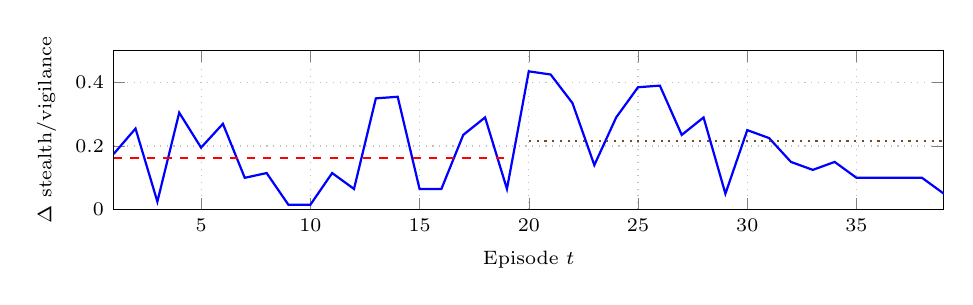
\begin{tikzpicture}
\begin{axis}[
  width=\columnwidth,
  height=3.6cm,
  xlabel={Episode $t$},
  ylabel={$\Delta$ stealth/vigilance},
  xmin=1, xmax=39,
  ymin=0, ymax=0.50,
  xticklabel style={font=\scriptsize},
  yticklabel style={font=\scriptsize},
  label style={font=\scriptsize},
  grid=major,
  major grid style={dotted,gray!50},
]
\addplot+[thick, mark=none] coordinates {(1,0.1750) (2,0.2550) (3,0.0250) (4,0.3050) (5,0.1950) (6,0.2700) (7,0.1000) (8,0.1150) (9,0.0150) (10,0.0150) (11,0.1150) (12,0.0650) (13,0.3500) (14,0.3550) (15,0.0650) (16,0.0650) (17,0.2350) (18,0.2900) (19,0.0650) (20,0.4350) (21,0.4250) (22,0.3350) (23,0.1400) (24,0.2900) (25,0.3850) (26,0.3900) (27,0.2350) (28,0.2900) (29,0.0500) (30,0.2500) (31,0.2250) (32,0.1500) (33,0.1250) (34,0.1500) (35,0.1000) (36,0.1000) (37,0.1000) (38,0.1000) (39,0.0500)};
\addplot+[thick, dashed, mark=none] coordinates {(1,0.1618) (19,0.1618)};
\addplot+[thick, dotted, mark=none] coordinates {(20,0.2162) (39,0.2162)};
\end{axis}
\end{tikzpicture}
\caption{Per-episode parameter change on a representative P/P run (seed~100). Parameter dynamics class: \emph{non convergent}. Distribution over all 54 ladder runs in Table~\ref{tab:dynamics}.}
\label{fig:arms}
\end{figure}
